\documentclass[letterpaper,11pt]{article}
\oddsidemargin -1.0cm \textwidth 17.5cm

\usepackage[utf8]{inputenc}
\usepackage[activeacute,spanish, es-lcroman]{babel}
\decimalpoint
\usepackage{amsfonts,setspace}
\usepackage{amsmath}
\usepackage{amssymb, amsmath, amsthm}
\usepackage{comment}
\usepackage{float}
\usepackage{amssymb}
\usepackage{dsfont}
\usepackage{anysize}
\usepackage{multicol}
\usepackage{enumerate}
\usepackage{graphicx}
\usepackage[left=1.5cm,top=2cm,right=1.5cm, bottom=1.7cm]{geometry}
\setlength\headheight{1.5em} 
\usepackage{fancyhdr}
\usepackage{multicol}
\usepackage{hyperref}
\usepackage{wrapfig}
\usepackage{subcaption}
\usepackage{siunitx}
\usepackage{cancel}
\usepackage{mdwlist}
\usepackage{svg}
\pagestyle{fancy}
\fancyhf{}
\renewcommand{\labelenumi}{\normalsize\bfseries P\arabic{enumi}.}
\renewcommand{\labelenumii}{\normalsize\bfseries (\alph{enumii})}
\renewcommand{\labelenumiii}{\normalsize\bfseries \roman{enumiii})}


\begin{document}

\fancyhead[L]{\itshape{Facultad de Ciencias F\'isicas y Matem\'aticas}}
\fancyhead[R]{\itshape{Universidad de Chile}}

\begin{minipage}{11.5cm}
    \begin{flushleft}
        \hspace*{-0.6cm}\textbf{FI1000-1 Introducción a la Física Clásica}\\
        \hspace*{-0.6cm}\textbf{Profesora:} Paulina Lira\\
        \hspace*{-0.6cm}\textbf{Auxiliares:} Alejandro Cartes \& Juan Cristóbal Castro\\
        \hspace*{-0.6cm}\textbf{Ayudantes:} Francisca Bórquez \& Catalina Molina\\
    \end{flushleft}
\end{minipage}

\begin{picture}(2,3)
    \put(366, 10){
\includegraphics[scale=0.9]{2020-1/Imágenes/logo/dfi-fcfm.pdf}}
\end{picture}

\begin{center}
	\LARGE\textbf{Auxiliar \#4}\\
	\Large{MCUA, mov. relativo y repaso C1}
\end{center}

\vspace{-1cm}
\begin{enumerate}\setlength{\itemsep}{0.4cm}

\rfoot[]{pág. \thepage}

\item[]

\item Un disco con un agujero a una distancia $R$ del centro está inicialmente en reposo. De repente, se lanza un proyectil verticalmente con velocidad $v_0$ de manera que pase por este agujero. Para que el proyectil logre caer en el mismo agujero, el disco comienza a girar con aceleración angular $\alpha$ constante inmediatamente cuando el proyectil pasa por este. Determine, en el instante en que el proyectil vuelve a pasar por el agujero:

\begin{multicols}{2}
    \begin{enumerate}
        \item $\alpha$ y la velocidad angular del disco
        
        \item la velocidad tangencial y el tamaño de la aceleración total que posee el agujero
    \end{enumerate}
    \columnbreak
    
    \begin{figure}[H]
        \centering
        \svgpath{../../2021-2/img/aux5}
        \includesvg[width=0.7\linewidth]{disco.svg}
    \end{figure}
    
\end{multicols}

\item Un tren se mueve sobre una línea recta horizontal con velocidad constante $v_0\hat{i}$. En un instante el maquinista lanza una maleta con velocidad $u_0\hat{j}$ verticalmente hacia arriba.

    \begin{enumerate}
        \item De acuerdo al maquinista, ¿cuál es la trayectoria de la maleta?
        
        \item Para un observador en reposo a un costado del tren, ¿cuál es el desplazamiento de la maleta desde que es lanzada hasta que cae de nuevo sobre el tren?
    \suspend{enumerate}
    
    Si ahora la maleta es lanzada por el maquinista con una velocidad $u = -v_0\hat{i} + n v_0\hat{j}$ y cada vagón del tren tiene una longitud $L$:
    
    \resume{enumerate}
        \item Bosqueje en el plano $x-y$ la trayectoria de la maleta registrada por un observador en reposo a un costado del tren.
        
        \item Determine el valor mínimo de $v_0$ para que la maleta caiga sobre el vagón k-ésimo.
        
    \end{enumerate}
    
\item Un anillo muy pequeño se hace girar con velocidad angular constante $\omega$ a lo largo de una circunferencia vertical de radio $R$. La circunferencia está cortada en un punto determinado por un ángulo $\theta = 30^{\circ}$, como se señala en la figura. Al alcanzar este punto, el anillo se desprende y continua en caída libre.

\begin{multicols}{2}
    \begin{enumerate}
        \item Calcule el valor de la velocidad angular $\omega$ si el anillo, luego de desprenderse, toca a la circunferencia precisamente en su punto más bajo $P$
    
        \item Para el caso anterior indique la velocidad y la rapidez del anillo cuando cruza el diámetro de la circunferencia (eje $x$)
    \end{enumerate}
    \columnbreak
    \begin{figure}[H]
        \centering
        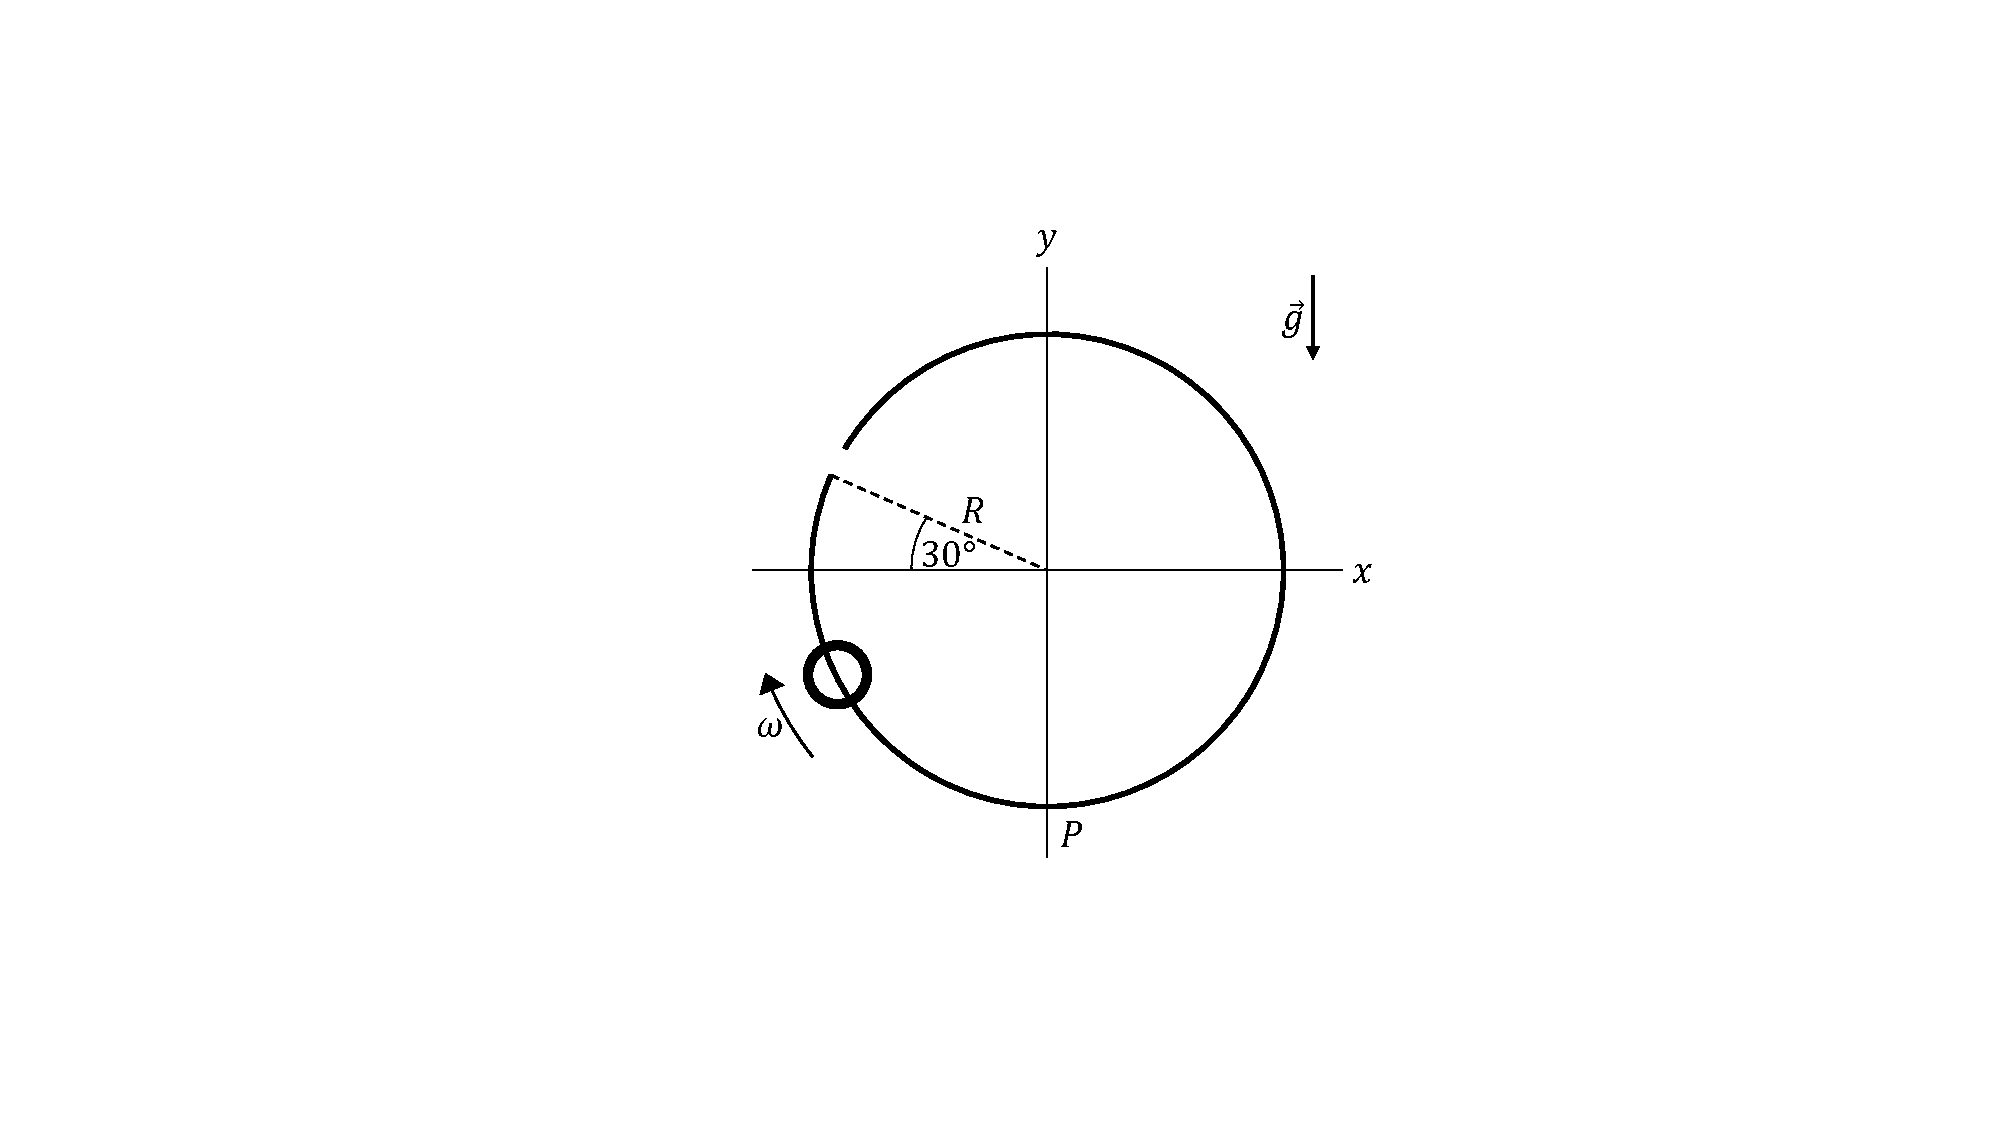
\includegraphics[scale = 0.40]{2020-1/Imágenes/aux4/circ_pelota.pdf}
    \end{figure}
\end{multicols}

\item Dos tortugas comienzan una carrera desde el punto $A$. Una de ellas viaja en línea recta desde el punto $A$ hasta el punto $B$ con aceleración constante $a_0$, partiendo del reposo. La otra tortuga lo hace describiendo una semicircunferencia de radio $R$, moviéndose con rapidez constante. Si ambas llegan al mismo tiempo al punto $B$, ¿cuál es la velocidad angular $\omega$ de la segunda tortuga?
    
\begin{figure}[H]
    \centering
    \svgpath{../../2021-2/img/aux3}
    \hspace{1em}
    \begin{subfigure}[t]{0.35\textwidth}
        \centering
        \includesvg[width=1\linewidth]{carrera.svg}
    \end{subfigure}
\end{figure}

\item Demuestre que para un proyectil disparado desde el suelo con un ángulo de lanzamiento \(\theta_0\) se cumple que:
\[\frac{H}{R} = \frac{1}{4}\tan{\theta_0}\]
donde $H$ es la altura máxima y $R$ es el alcance horizontal máximo


% Para imágenes vectoriales -> el texto tiene que estar en LaTeX
% \begin{figure}[htbp]
%   \centering
%   \svgpath{../Imagenes/ejercicios}  -> .. irse pa'trás 
%   \includesvg{ej5.svg}
% \end{figure}

\end{enumerate}
\end{document}
